% ! TeX root = main.tex

\begin{frame}{Background}
  \begin{backgroundblock} 
    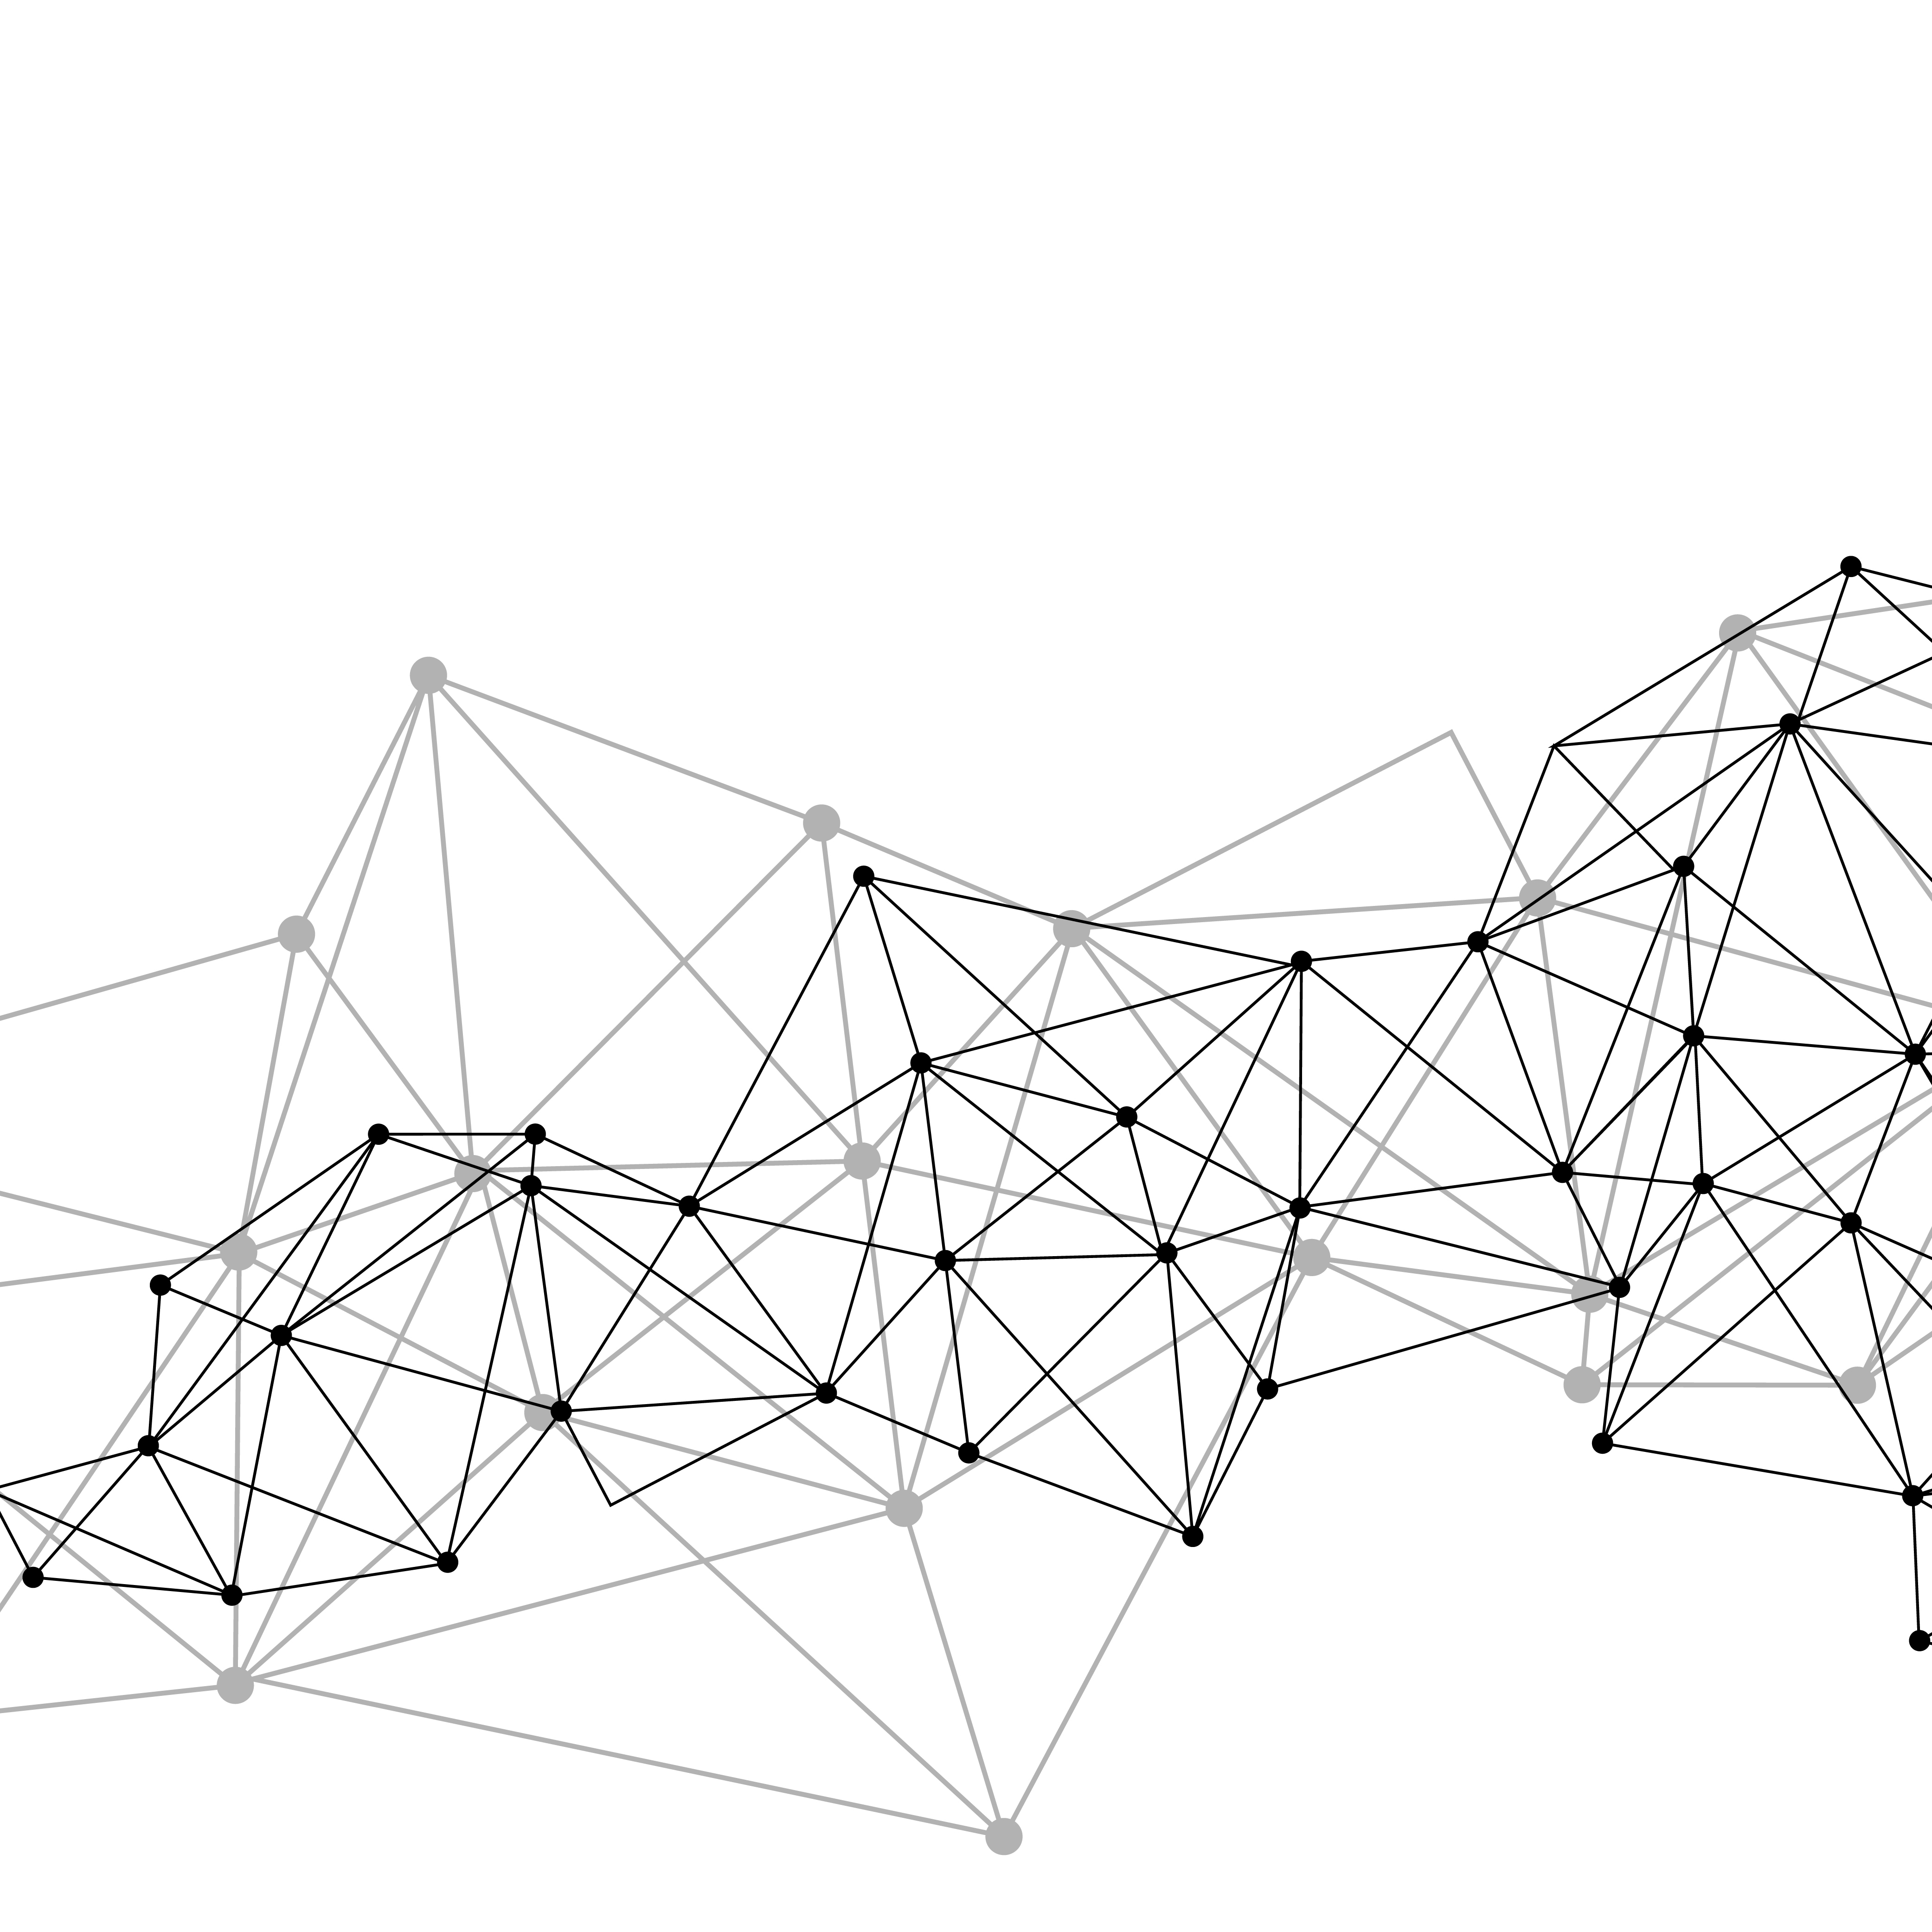
\includegraphics[width=\paperwidth]{img/main-background.jpg} 
  \end{backgroundblock} 
  \begin{card}[Collective (Self-)Adaptive Systems (\textbf{CSAS})]
    {
      \color{accent}
      Distributed and interconnected systems composed of multiple agents that can perform complex 
      tasks exhibiting robust collective behaviours while achieve system-wide and agent-specific goal. 
    }

  \pdfcomment{
    Our research effort consists of an engineering Collective (Self-)Adaptive System. 
    They can be defined as distributed and interconnected systems composed of multiple agents that can perform complex 
    tasks such as environmental data collection, search and rescue operations, and discovery of natural resources.
    So the collective exhibit robust behaviour while achieving system-wide and agent-specific goals.
    For years, there have been various approaches in the literature to deal with these systems. 
    In my research group, we focus on Aggregate Computing.
  }
  \end{card}
\end{frame}